%!TEX root = ../thesis.tex
%*******************************************************************************
%****************************** Third Chapter **********************************
%*******************************************************************************
\chapter{Predicting \mtb{} drug resistance}
\label{chap:dst}
% **************************** Define Graphics Path **************************
\ifpdf
    \graphicspath{{Chapter3/Figs/Raster/}{Chapter3/Figs/PDF/}{Chapter3/Figs/}}
\else
    \graphicspath{{Chapter3/Figs/Vector/}{Chapter3/Figs/}}
\fi

%=========================================================================
%=========================================================================

\setcounter{section}{-1}
\section{Publication and collaboration acknowledgements}
\label{sec:ch3-acknowledge}

%=========================================================================
\section{Introduction}

%=========================================================================
\section{Dataset}
% refer to previous chapter for sequencing info and mention we use the samples that passed QC

\subsection{DST}
% I have asked the collaborators for the DST methods

% add the upset plot summarising the available phenotype data
% also add a table with the raw numbers for the upset plot
\begin{figure}
\begin{center}
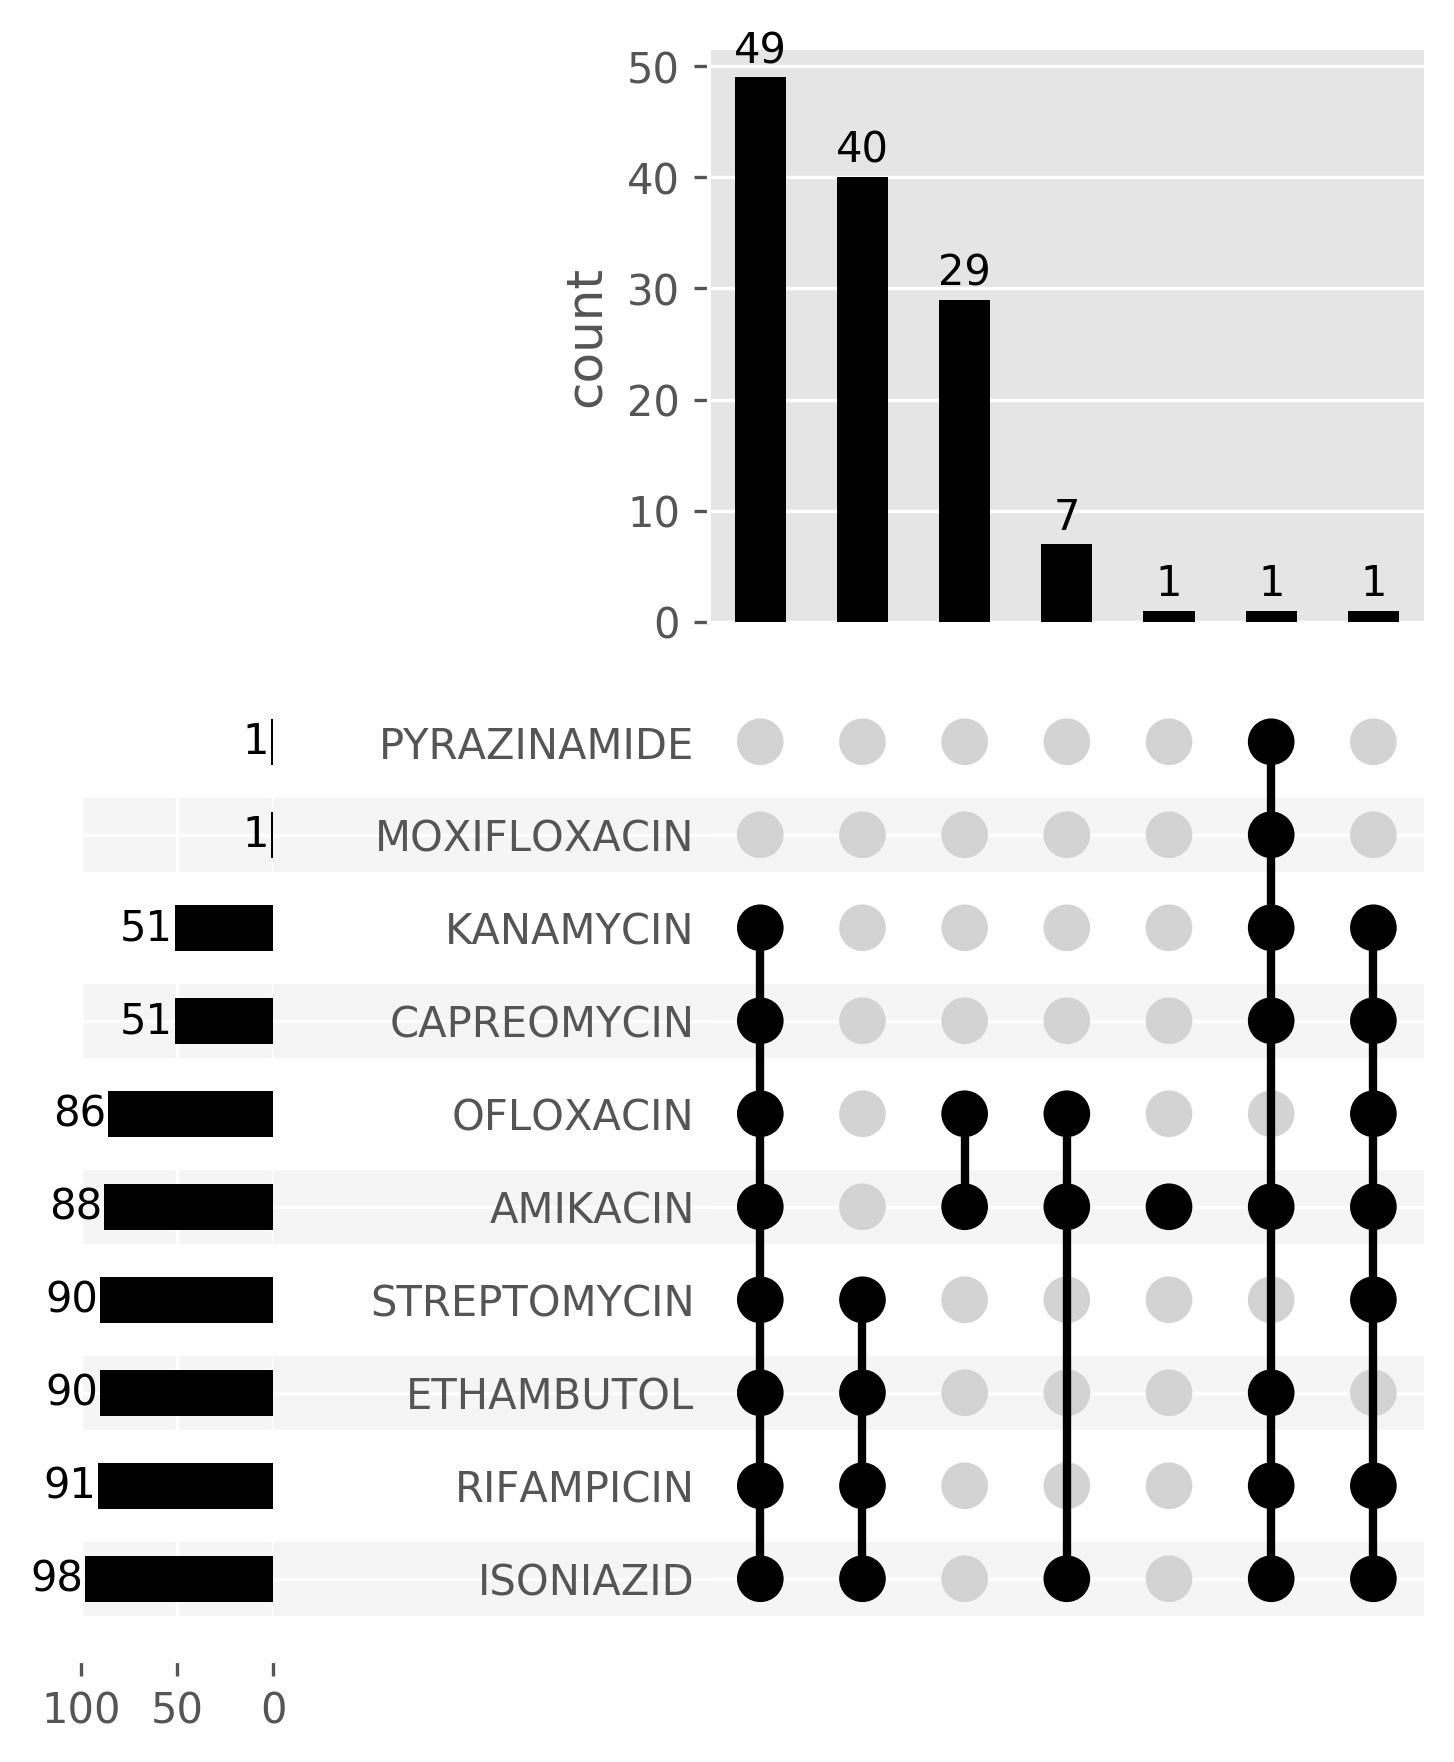
\includegraphics[width=0.90\columnwidth]{Chapter3/Figs/available_dst.png}
\caption{{Culture-based drug susceptibility data available for samples. Each row is a drug, and the columns represent a set of samples that have phenotype information for those drugs with a filled cell. The top panel shows the number of samples in the set for that combination of drugs. The bar plot in the left panel shows the number of samples with phenotype information for that drug.
{\label{fig:available-dst}}
}}
\end{center}
\end{figure}
%=========================================================================
\section{Drug resistance prediction with genome graphs}
% i.e., methods for drprg

\subsection{Constructing a panel reference graph}
% also add in some examples of crazy sites that lead to the change in construction method

\subsection{Predictions}
% how we go from reads and panel to predictions
% also outline what we do with novel stuff

%=========================================================================
\section{Concordance with phenotype}
%  alot of FP ethambutol are M306 mutation which is strongly associated with resistance https://europepmc.org/article/PMC/4505224

\begin{figure}
\begin{center}
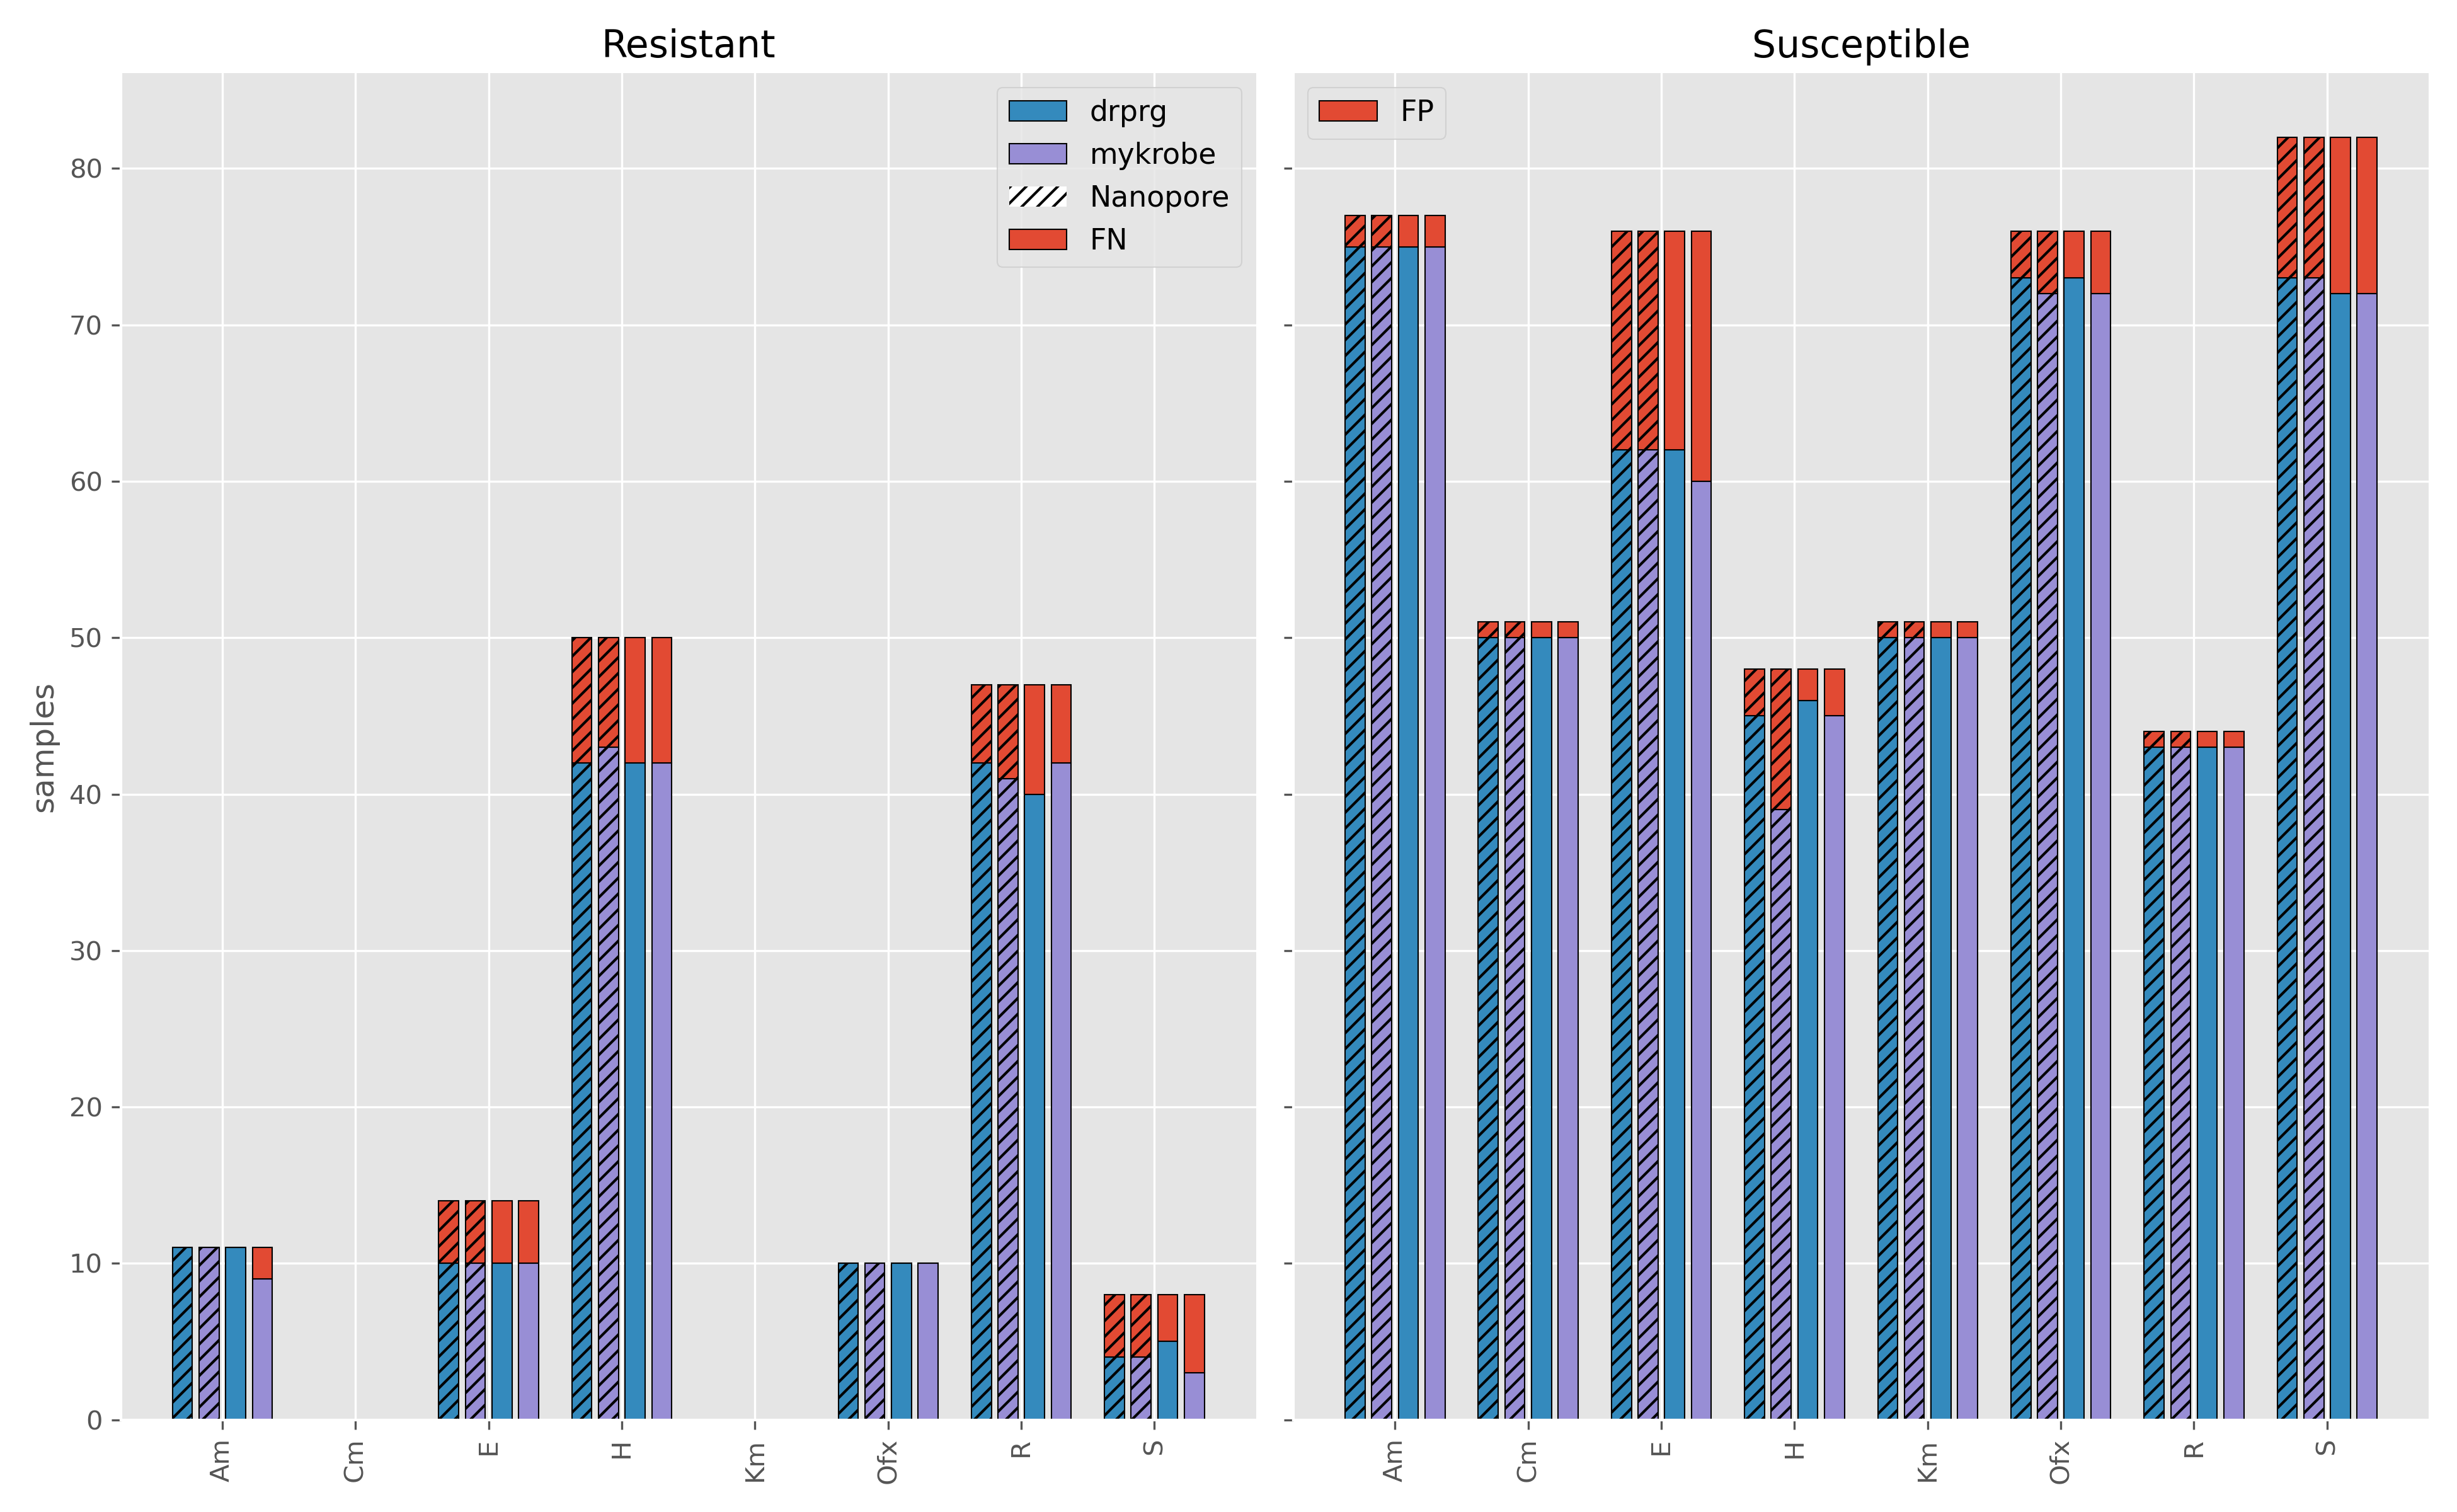
\includegraphics[width=0.90\columnwidth]{Chapter3/Figs/phenotype_concordance.png}
\caption{{Number of resistant (left) and susceptible (right) phenotypes correctly identified by mykrobe from Illumina (blue) and Nanopore (purple) data from the same samples. The red bars indicate missed (FN) or incorrect (FP) predictions. The x-axis shows the drugs with available phenotype data that mykrobe also makes predictions for. E - ethambutol; H - isoniazid; Z - pyrazinamide; R - rifampicin; S - streptomycin; Km - kanamycin; Am - amikacin; Ofx - ofloxacin; Cm - capreomycin; Mfx - moxifloxacin.
{\label{fig:pheno-concordance}}
}}
\end{center}
\end{figure}

% Please add the following required packages to your document preamble:
% \usepackage{multirow}
% \usepackage{graphicx}
\begin{table}
\centering
\resizebox{\textwidth}{!}{%
\begin{tabular}{|l|l|l|c|c|c|c|c|c|}
\hline
Drug                           & Technology                 & Tool                          & FN(R)                         & FP(S)                          & FNR(95\% CI)                                 & FPR(95\% CI)                                 & PPV(95\% CI)                                 & NPV(95\% CI)                                   \\ \hline
                               &                            & \cellcolor[HTML]{EFEFEF}Drprg & \cellcolor[HTML]{EFEFEF}0(11) & \cellcolor[HTML]{EFEFEF}2(77)  & \cellcolor[HTML]{EFEFEF}0.0\% (0.0-25.9\%)   & \cellcolor[HTML]{EFEFEF}2.6\% (0.7-9.0\%)    & \cellcolor[HTML]{EFEFEF}84.6\% (57.8-95.7\%) & \cellcolor[HTML]{EFEFEF}100.0\% (95.1-100.0\%) \\ \cline{3-9} 
                               & \multirow{-2}{*}{Illumina} & Mykrobe                       & 0(11)                         & 2(77)                          & 0.0\% (0.0-25.9\%)                           & 2.6\% (0.7-9.0\%)                            & 84.6\% (57.8-95.7\%)                         & 100.0\% (95.1-100.0\%)                         \\ \cline{2-9} 
                               &                            & \cellcolor[HTML]{EFEFEF}Drprg & \cellcolor[HTML]{EFEFEF}0(11) & \cellcolor[HTML]{EFEFEF}2(77)  & \cellcolor[HTML]{EFEFEF}0.0\% (0.0-25.9\%)   & \cellcolor[HTML]{EFEFEF}2.6\% (0.7-9.0\%)    & \cellcolor[HTML]{EFEFEF}84.6\% (57.8-95.7\%) & \cellcolor[HTML]{EFEFEF}100.0\% (95.1-100.0\%) \\ \cline{3-9} 
\multirow{-4}{*}{Amikacin}     & \multirow{-2}{*}{Nanopore} & Mykrobe                       & 2(11)                         & 2(77)                          & 18.2\% (5.1-47.7\%)                          & 2.6\% (0.7-9.0\%)                            & 81.8\% (52.3-94.9\%)                         & 97.4\% (91.0-99.3\%)                           \\ \hline
                               &                            & \cellcolor[HTML]{EFEFEF}Drprg & \cellcolor[HTML]{EFEFEF}0(0)  & \cellcolor[HTML]{EFEFEF}1(51)  & \cellcolor[HTML]{EFEFEF}-                    & \cellcolor[HTML]{EFEFEF}2.0\% (0.3-10.3\%)   & \cellcolor[HTML]{EFEFEF}0.0\% (0.0-79.3\%)   & \cellcolor[HTML]{EFEFEF}100.0\% (92.9-100.0\%) \\ \cline{3-9} 
                               & \multirow{-2}{*}{Illumina} & Mykrobe                       & 0(0)                          & 1(51)                          & -                                            & 2.0\% (0.3-10.3\%)                           & 0.0\% (0.0-79.3\%)                           & 100.0\% (92.9-100.0\%)                         \\ \cline{2-9} 
                               &                            & \cellcolor[HTML]{EFEFEF}Drprg & \cellcolor[HTML]{EFEFEF}0(0)  & \cellcolor[HTML]{EFEFEF}1(51)  & \cellcolor[HTML]{EFEFEF}-                    & \cellcolor[HTML]{EFEFEF}2.0\% (0.3-10.3\%)   & \cellcolor[HTML]{EFEFEF}0.0\% (0.0-79.3\%)   & \cellcolor[HTML]{EFEFEF}100.0\% (92.9-100.0\%) \\ \cline{3-9} 
\multirow{-4}{*}{Capreomycin}  & \multirow{-2}{*}{Nanopore} & Mykrobe                       & 0(0)                          & 1(51)                          & -                                            & 2.0\% (0.3-10.3\%)                           & 0.0\% (0.0-79.3\%)                           & 100.0\% (92.9-100.0\%)                         \\ \hline
                               &                            & \cellcolor[HTML]{EFEFEF}Drprg & \cellcolor[HTML]{EFEFEF}4(14) & \cellcolor[HTML]{EFEFEF}14(76) & \cellcolor[HTML]{EFEFEF}28.6\% (11.7-54.6\%) & \cellcolor[HTML]{EFEFEF}18.4\% (11.3-28.6\%) & \cellcolor[HTML]{EFEFEF}41.7\% (24.5-61.2\%) & \cellcolor[HTML]{EFEFEF}93.9\% (85.4-97.6\%)   \\ \cline{3-9} 
                               & \multirow{-2}{*}{Illumina} & Mykrobe                       & 4(14)                         & 14(76)                         & 28.6\% (11.7-54.6\%)                         & 18.4\% (11.3-28.6\%)                         & 41.7\% (24.5-61.2\%)                         & 93.9\% (85.4-97.6\%)                           \\ \cline{2-9} 
                               &                            & \cellcolor[HTML]{EFEFEF}Drprg & \cellcolor[HTML]{EFEFEF}4(14) & \cellcolor[HTML]{EFEFEF}14(76) & \cellcolor[HTML]{EFEFEF}28.6\% (11.7-54.6\%) & \cellcolor[HTML]{EFEFEF}18.4\% (11.3-28.6\%) & \cellcolor[HTML]{EFEFEF}41.7\% (24.5-61.2\%) & \cellcolor[HTML]{EFEFEF}93.9\% (85.4-97.6\%)   \\ \cline{3-9} 
\multirow{-4}{*}{Ethambutol}   & \multirow{-2}{*}{Nanopore} & Mykrobe                       & 4(14)                         & 16(76)                         & 28.6\% (11.7-54.6\%)                         & 21.1\% (13.4-31.5\%)                         & 38.5\% (22.4-57.5\%)                         & 93.8\% (85.0-97.5\%)                           \\ \hline
                               &                            & \cellcolor[HTML]{EFEFEF}Drprg & \cellcolor[HTML]{EFEFEF}8(50) & \cellcolor[HTML]{EFEFEF}3(48)  & \cellcolor[HTML]{EFEFEF}16.0\% (8.3-28.5\%)  & \cellcolor[HTML]{EFEFEF}6.2\% (2.1-16.8\%)   & \cellcolor[HTML]{EFEFEF}93.3\% (82.1-97.7\%) & \cellcolor[HTML]{EFEFEF}84.9\% (72.9-92.1\%)   \\ \cline{3-9} 
                               & \multirow{-2}{*}{Illumina} & Mykrobe                       & 7(50)                         & 9(48)                          & 14.0\% (7.0-26.2\%)                          & 18.8\% (10.2-31.9\%)                         & 82.7\% (70.3-90.6\%)                         & 84.8\% (71.8-92.4\%)                           \\ \cline{2-9} 
                               &                            & \cellcolor[HTML]{EFEFEF}Drprg & \cellcolor[HTML]{EFEFEF}8(50) & \cellcolor[HTML]{EFEFEF}2(48)  & \cellcolor[HTML]{EFEFEF}16.0\% (8.3-28.5\%)  & \cellcolor[HTML]{EFEFEF}4.2\% (1.2-14.0\%)   & \cellcolor[HTML]{EFEFEF}95.5\% (84.9-98.7\%) & \cellcolor[HTML]{EFEFEF}85.2\% (73.4-92.3\%)   \\ \cline{3-9} 
\multirow{-4}{*}{Isoniazid}    & \multirow{-2}{*}{Nanopore} & Mykrobe                       & 8(50)                         & 3(48)                          & 16.0\% (8.3-28.5\%)                          & 6.2\% (2.1-16.8\%)                           & 93.3\% (82.1-97.7\%)                         & 84.9\% (72.9-92.1\%)                           \\ \hline
                               &                            & \cellcolor[HTML]{EFEFEF}Drprg & \cellcolor[HTML]{EFEFEF}0(0)  & \cellcolor[HTML]{EFEFEF}1(51)  & \cellcolor[HTML]{EFEFEF}-                    & \cellcolor[HTML]{EFEFEF}2.0\% (0.3-10.3\%)   & \cellcolor[HTML]{EFEFEF}0.0\% (0.0-79.3\%)   & \cellcolor[HTML]{EFEFEF}100.0\% (92.9-100.0\%) \\ \cline{3-9} 
                               & \multirow{-2}{*}{Illumina} & Mykrobe                       & 0(0)                          & 1(51)                          & -                                            & 2.0\% (0.3-10.3\%)                           & 0.0\% (0.0-79.3\%)                           & 100.0\% (92.9-100.0\%)                         \\ \cline{2-9} 
                               &                            & \cellcolor[HTML]{EFEFEF}Drprg & \cellcolor[HTML]{EFEFEF}0(0)  & \cellcolor[HTML]{EFEFEF}1(51)  & \cellcolor[HTML]{EFEFEF}-                    & \cellcolor[HTML]{EFEFEF}2.0\% (0.3-10.3\%)   & \cellcolor[HTML]{EFEFEF}0.0\% (0.0-79.3\%)   & \cellcolor[HTML]{EFEFEF}100.0\% (92.9-100.0\%) \\ \cline{3-9} 
\multirow{-4}{*}{Kanamycin}    & \multirow{-2}{*}{Nanopore} & Mykrobe                       & 0(0)                          & 1(51)                          & -                                            & 2.0\% (0.3-10.3\%)                           & 0.0\% (0.0-79.3\%)                           & 100.0\% (92.9-100.0\%)                         \\ \hline
                               &                            & \cellcolor[HTML]{EFEFEF}Drprg & \cellcolor[HTML]{EFEFEF}0(10) & \cellcolor[HTML]{EFEFEF}3(76)  & \cellcolor[HTML]{EFEFEF}0.0\% (-0.0-27.8\%)  & \cellcolor[HTML]{EFEFEF}3.9\% (1.4-11.0\%)   & \cellcolor[HTML]{EFEFEF}76.9\% (49.7-91.8\%) & \cellcolor[HTML]{EFEFEF}100.0\% (95.0-100.0\%) \\ \cline{3-9} 
                               & \multirow{-2}{*}{Illumina} & Mykrobe                       & 0(10)                         & 4(76)                          & 0.0\% (-0.0-27.8\%)                          & 5.3\% (2.1-12.8\%)                           & 71.4\% (45.4-88.3\%)                         & 100.0\% (94.9-100.0\%)                         \\ \cline{2-9} 
                               &                            & \cellcolor[HTML]{EFEFEF}Drprg & \cellcolor[HTML]{EFEFEF}0(10) & \cellcolor[HTML]{EFEFEF}3(76)  & \cellcolor[HTML]{EFEFEF}0.0\% (-0.0-27.8\%)  & \cellcolor[HTML]{EFEFEF}3.9\% (1.4-11.0\%)   & \cellcolor[HTML]{EFEFEF}76.9\% (49.7-91.8\%) & \cellcolor[HTML]{EFEFEF}100.0\% (95.0-100.0\%) \\ \cline{3-9} 
\multirow{-4}{*}{Ofloxacin}    & \multirow{-2}{*}{Nanopore} & Mykrobe                       & 0(10)                         & 4(76)                          & 0.0\% (-0.0-27.8\%)                          & 5.3\% (2.1-12.8\%)                           & 71.4\% (45.4-88.3\%)                         & 100.0\% (94.9-100.0\%)                         \\ \hline
                               &                            & \cellcolor[HTML]{EFEFEF}Drprg & \cellcolor[HTML]{EFEFEF}5(47) & \cellcolor[HTML]{EFEFEF}1(44)  & \cellcolor[HTML]{EFEFEF}10.6\% (4.6-22.6\%)  & \cellcolor[HTML]{EFEFEF}2.3\% (0.4-11.8\%)   & \cellcolor[HTML]{EFEFEF}97.7\% (87.9-99.6\%) & \cellcolor[HTML]{EFEFEF}89.6\% (77.8-95.5\%)   \\ \cline{3-9} 
                               & \multirow{-2}{*}{Illumina} & Mykrobe                       & 6(47)                         & 1(44)                          & 12.8\% (6.0-25.2\%)                          & 2.3\% (0.4-11.8\%)                           & 97.6\% (87.7-99.6\%)                         & 87.8\% (75.8-94.3\%)                           \\ \cline{2-9} 
                               &                            & \cellcolor[HTML]{EFEFEF}Drprg & \cellcolor[HTML]{EFEFEF}7(47) & \cellcolor[HTML]{EFEFEF}1(44)  & \cellcolor[HTML]{EFEFEF}14.9\% (7.4-27.7\%)  & \cellcolor[HTML]{EFEFEF}2.3\% (0.4-11.8\%)   & \cellcolor[HTML]{EFEFEF}97.6\% (87.4-99.6\%) & \cellcolor[HTML]{EFEFEF}86.0\% (73.8-93.0\%)   \\ \cline{3-9} 
\multirow{-4}{*}{Rifampicin}   & \multirow{-2}{*}{Nanopore} & Mykrobe                       & 5(47)                         & 1(44)                          & 10.6\% (4.6-22.6\%)                          & 2.3\% (0.4-11.8\%)                           & 97.7\% (87.9-99.6\%)                         & 89.6\% (77.8-95.5\%)                           \\ \hline
                               &                            & \cellcolor[HTML]{EFEFEF}Drprg & \cellcolor[HTML]{EFEFEF}4(8)  & \cellcolor[HTML]{EFEFEF}9(82)  & \cellcolor[HTML]{EFEFEF}50.0\% (21.5-78.5\%) & \cellcolor[HTML]{EFEFEF}11.0\% (5.9-19.6\%)  & \cellcolor[HTML]{EFEFEF}30.8\% (12.7-57.6\%) & \cellcolor[HTML]{EFEFEF}94.8\% (87.4-98.0\%)   \\ \cline{3-9} 
                               & \multirow{-2}{*}{Illumina} & Mykrobe                       & 4(8)                          & 9(82)                          & 50.0\% (21.5-78.5\%)                         & 11.0\% (5.9-19.6\%)                          & 30.8\% (12.7-57.6\%)                         & 94.8\% (87.4-98.0\%)                           \\ \cline{2-9} 
                               &                            & \cellcolor[HTML]{EFEFEF}Drprg & \cellcolor[HTML]{EFEFEF}3(8)  & \cellcolor[HTML]{EFEFEF}10(82) & \cellcolor[HTML]{EFEFEF}37.5\% (13.7-69.4\%) & \cellcolor[HTML]{EFEFEF}12.2\% (6.8-21.0\%)  & \cellcolor[HTML]{EFEFEF}33.3\% (15.2-58.3\%) & \cellcolor[HTML]{EFEFEF}96.0\% (88.9-98.6\%)   \\ \cline{3-9} 
\multirow{-4}{*}{Streptomycin} & \multirow{-2}{*}{Nanopore} & Mykrobe                       & 5(8)                          & 10(82)                         & 62.5\% (30.6-86.3\%)                         & 12.2\% (6.8-21.0\%)                          & 23.1\% (8.2-50.3\%)                          & 93.5\% (85.7-97.2\%)                           \\ \cline{3-9} 
\end{tabular}%
}
\caption{Comparison of drug resistance predictions with culture-based phenotype.
For this comparison, we assume the drug susceptibility testing phenotype is correct and evaluate mykrobe Illumina and Nanopore resistance predictions accordingly. Pyrazinamide and Moxifloxacin are excluded as phenotype information is only available for 1 sample.
FN=false negative; R=number of resistant samples; FP=false positive; S=number of susceptible samples; FNR=false negative rate; FPR=false positive rate; PPV=positive predictive value; NPV=negative predictive value; CI=Wilson score confidence interval}
\label{tab:pheno-concordance}
\end{table}
%=========================================================================
\section{Concordance with Illumina}

\begin{figure}
\begin{center}
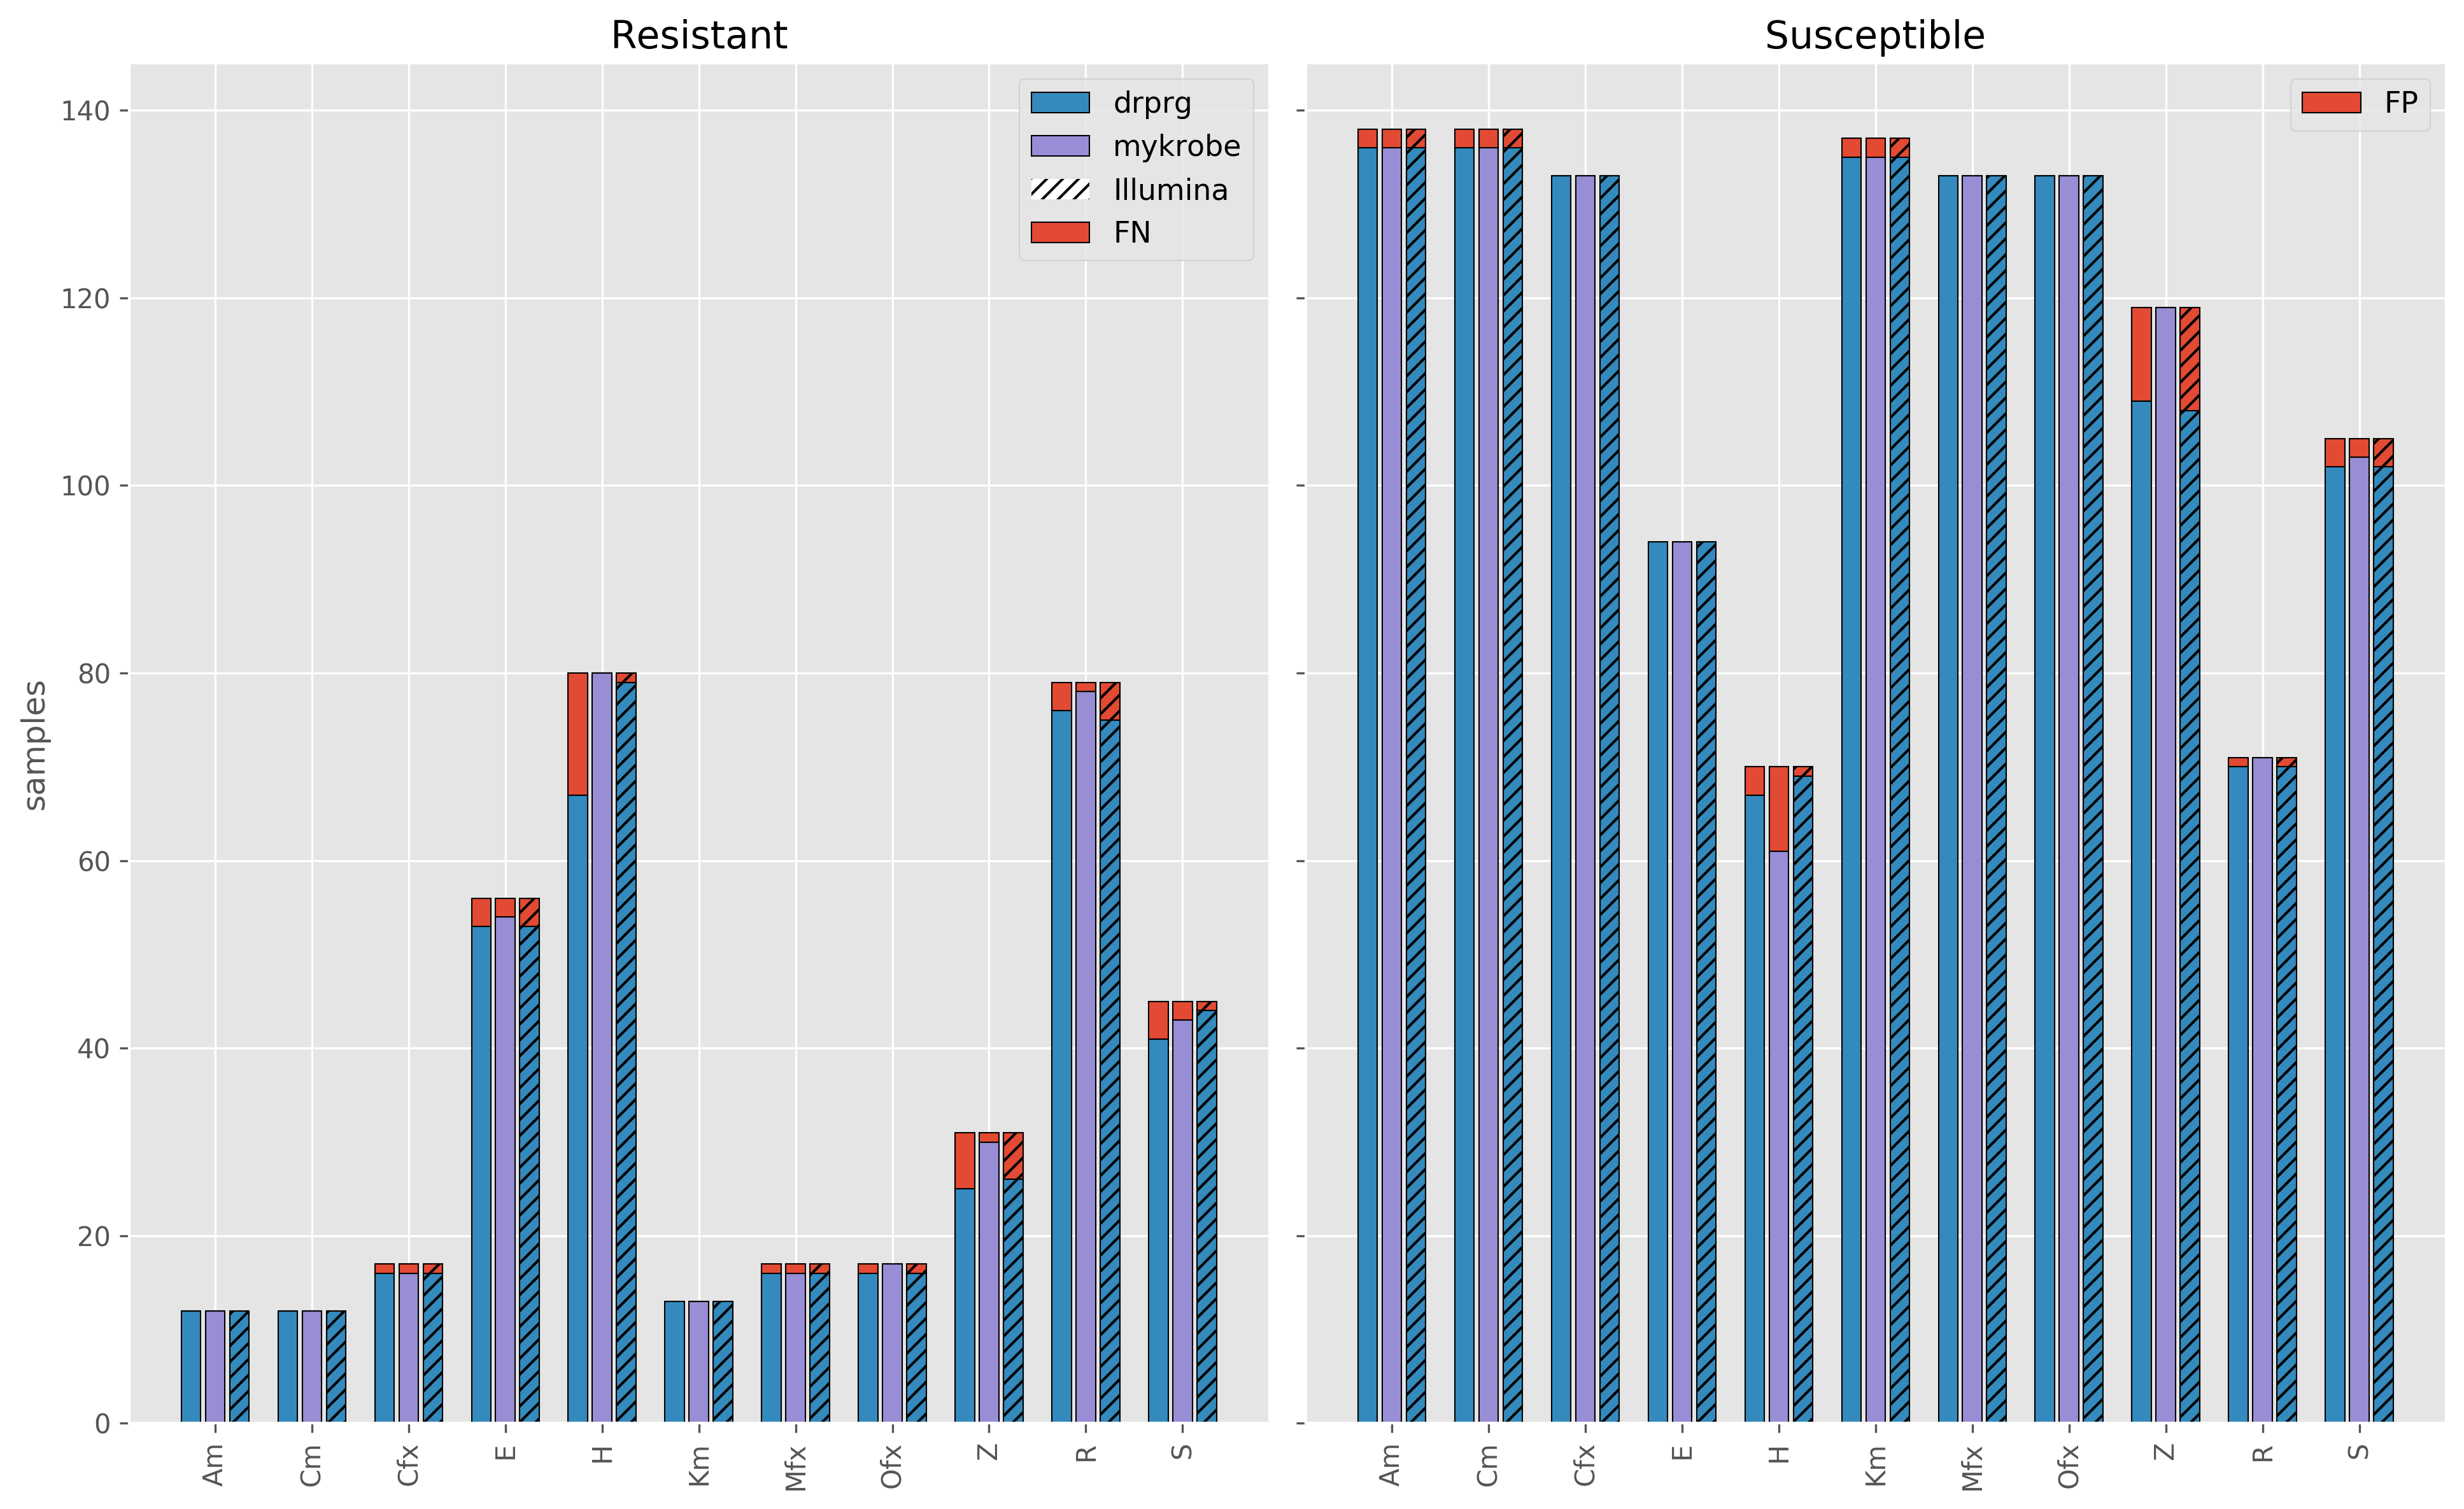
\includegraphics[width=0.90\columnwidth]{Chapter3/Figs/illumina_concordance.png}
\caption{{Number of resistant (left) and susceptible (right) genotypes correctly identified by mykrobe from Illumina (blue) and Nanopore (purple) data from the same samples. The genotypes are predictions from mykrobe with Illumina data. The red bars indicate missed (FN) or incorrect (FP) predictions. The x-axis shows the drugs with available phenotype data that mykrobe also makes predictions for. E - ethambutol; H - isoniazid; Z - pyrazinamide; R - rifampicin; S - streptomycin; Km - kanamycin; Am - amikacin; Ofx - ofloxacin; Cm - capreomycin; Mfx - moxifloxacin.
{\label{fig:geno-concordance}}
}}
\end{center}
\end{figure}

% Please add the following required packages to your document preamble:
% \usepackage{multirow}
% \usepackage{graphicx}
\begin{table}
\centering
\resizebox{\textwidth}{!}{%
\begin{tabular}{|l|l|l|c|c|c|c|c|c|}
\hline
Drug                            & Tool                    & Technology                 & FN(R)                          & FP(S)                           & FNR(95\% CI)                                & FPR(95\% CI)                                & PPV(95\% CI)                                   & NPV(95\% CI)                                   \\ \hline
                                &                         & Illumina                   & \cellcolor[HTML]{EFEFEF}0(12)  & \cellcolor[HTML]{EFEFEF}2(138)  & \cellcolor[HTML]{EFEFEF}0.0\% (0.0-24.2\%)  & \cellcolor[HTML]{EFEFEF}1.4\% (0.4-5.1\%)   & \cellcolor[HTML]{EFEFEF}85.7\% (60.1-96.0\%)   & \cellcolor[HTML]{EFEFEF}100.0\% (97.3-100.0\%) \\ \cline{3-9} 
                                & \multirow{-2}{*}{Drprg} &                            & 0(12)                          & 2(138)                          & 0.0\% (0.0-24.2\%)                          & 1.4\% (0.4-5.1\%)                           & 85.7\% (60.1-96.0\%)                           & 100.0\% (97.3-100.0\%)                         \\ \cline{2-2} \cline{4-9} 
\multirow{-3}{*}{Amikacin}      & Mykrobe                 & \multirow{-2}{*}{Nanopore} & \cellcolor[HTML]{EFEFEF}0(12)  & \cellcolor[HTML]{EFEFEF}2(138)  & \cellcolor[HTML]{EFEFEF}0.0\% (0.0-24.2\%)  & \cellcolor[HTML]{EFEFEF}1.4\% (0.4-5.1\%)   & \cellcolor[HTML]{EFEFEF}85.7\% (60.1-96.0\%)   & \cellcolor[HTML]{EFEFEF}100.0\% (97.3-100.0\%) \\ \hline
                                &                         & Illumina                   & 0(12)                          & 2(138)                          & 0.0\% (0.0-24.2\%)                          & 1.4\% (0.4-5.1\%)                           & 85.7\% (60.1-96.0\%)                           & 100.0\% (97.3-100.0\%)                         \\ \cline{3-9} 
                                & \multirow{-2}{*}{Drprg} &                            & \cellcolor[HTML]{EFEFEF}0(12)  & \cellcolor[HTML]{EFEFEF}2(138)  & \cellcolor[HTML]{EFEFEF}0.0\% (0.0-24.2\%)  & \cellcolor[HTML]{EFEFEF}1.4\% (0.4-5.1\%)   & \cellcolor[HTML]{EFEFEF}85.7\% (60.1-96.0\%)   & \cellcolor[HTML]{EFEFEF}100.0\% (97.3-100.0\%) \\ \cline{2-2} \cline{4-9} 
\multirow{-3}{*}{Capreomycin}   & Mykrobe                 & \multirow{-2}{*}{Nanopore} & 0(12)                          & 2(138)                          & 0.0\% (0.0-24.2\%)                          & 1.4\% (0.4-5.1\%)                           & 85.7\% (60.1-96.0\%)                           & 100.0\% (97.3-100.0\%)                         \\ \hline
                                &                         & Illumina                   & \cellcolor[HTML]{EFEFEF}1(17)  & \cellcolor[HTML]{EFEFEF}0(133)  & \cellcolor[HTML]{EFEFEF}5.9\% (1.0-27.0\%)  & \cellcolor[HTML]{EFEFEF}0.0\% (0.0-2.8\%)   & \cellcolor[HTML]{EFEFEF}100.0\% (80.6-100.0\%) & \cellcolor[HTML]{EFEFEF}99.3\% (95.9-99.9\%)   \\ \cline{3-9} 
                                & \multirow{-2}{*}{Drprg} &                            & 1(17)                          & 0(133)                          & 5.9\% (1.0-27.0\%)                          & 0.0\% (0.0-2.8\%)                           & 100.0\% (80.6-100.0\%)                         & 99.3\% (95.9-99.9\%)                           \\ \cline{2-2} \cline{4-9} 
\multirow{-3}{*}{Ciprofloxacin} & Mykrobe                 & \multirow{-2}{*}{Nanopore} & \cellcolor[HTML]{EFEFEF}1(17)  & \cellcolor[HTML]{EFEFEF}0(133)  & \cellcolor[HTML]{EFEFEF}5.9\% (1.0-27.0\%)  & \cellcolor[HTML]{EFEFEF}0.0\% (0.0-2.8\%)   & \cellcolor[HTML]{EFEFEF}100.0\% (80.6-100.0\%) & \cellcolor[HTML]{EFEFEF}99.3\% (95.9-99.9\%)   \\ \hline
                                &                         & Illumina                   & 3(56)                          & 0(94)                           & 5.4\% (1.8-14.6\%)                          & 0.0\% (0.0-3.9\%)                           & 100.0\% (93.2-100.0\%)                         & 96.9\% (91.3-98.9\%)                           \\ \cline{3-9} 
                                & \multirow{-2}{*}{Drprg} &                            & \cellcolor[HTML]{EFEFEF}2(56)  & \cellcolor[HTML]{EFEFEF}0(94)   & \cellcolor[HTML]{EFEFEF}3.6\% (1.0-12.1\%)  & \cellcolor[HTML]{EFEFEF}0.0\% (0.0-3.9\%)   & \cellcolor[HTML]{EFEFEF}100.0\% (93.4-100.0\%) & \cellcolor[HTML]{EFEFEF}97.9\% (92.7-99.4\%)   \\ \cline{2-2} \cline{4-9} 
\multirow{-3}{*}{Ethambutol}    & Mykrobe                 & \multirow{-2}{*}{Nanopore} & 3(56)                          & 0(94)                           & 5.4\% (1.8-14.6\%)                          & 0.0\% (0.0-3.9\%)                           & 100.0\% (93.2-100.0\%)                         & 96.9\% (91.3-98.9\%)                           \\ \hline
                                &                         & Illumina                   & \cellcolor[HTML]{EFEFEF}10(80) & \cellcolor[HTML]{EFEFEF}6(70)   & \cellcolor[HTML]{EFEFEF}12.5\% (6.9-21.5\%) & \cellcolor[HTML]{EFEFEF}8.6\% (4.0-17.5\%)  & \cellcolor[HTML]{EFEFEF}92.1\% (83.8-96.3\%)   & \cellcolor[HTML]{EFEFEF}86.5\% (76.9-92.5\%)   \\ \cline{3-9} 
                                & \multirow{-2}{*}{Drprg} &                            & 0(80)                          & 9(70)                           & 0.0\% (0.0-4.6\%)                           & 12.9\% (6.9-22.7\%)                         & 89.9\% (81.9-94.6\%)                           & 100.0\% (94.1-100.0\%)                         \\ \cline{2-2} \cline{4-9} 
\multirow{-3}{*}{Isoniazid}     & Mykrobe                 & \multirow{-2}{*}{Nanopore} & \cellcolor[HTML]{EFEFEF}1(80)  & \cellcolor[HTML]{EFEFEF}1(70)   & \cellcolor[HTML]{EFEFEF}1.2\% (0.2-6.7\%)   & \cellcolor[HTML]{EFEFEF}1.4\% (0.3-7.7\%)   & \cellcolor[HTML]{EFEFEF}98.8\% (93.3-99.8\%)   & \cellcolor[HTML]{EFEFEF}98.6\% (92.3-99.7\%)   \\ \hline
                                &                         & Illumina                   & 0(13)                          & 2(137)                          & 0.0\% (0.0-22.8\%)                          & 1.5\% (0.4-5.2\%)                           & 86.7\% (62.1-96.3\%)                           & 100.0\% (97.2-100.0\%)                         \\ \cline{3-9} 
                                & \multirow{-2}{*}{Drprg} &                            & \cellcolor[HTML]{EFEFEF}0(13)  & \cellcolor[HTML]{EFEFEF}2(137)  & \cellcolor[HTML]{EFEFEF}0.0\% (0.0-22.8\%)  & \cellcolor[HTML]{EFEFEF}1.5\% (0.4-5.2\%)   & \cellcolor[HTML]{EFEFEF}86.7\% (62.1-96.3\%)   & \cellcolor[HTML]{EFEFEF}100.0\% (97.2-100.0\%) \\ \cline{2-2} \cline{4-9} 
\multirow{-3}{*}{Kanamycin}     & Mykrobe                 & \multirow{-2}{*}{Nanopore} & 0(13)                          & 2(137)                          & 0.0\% (0.0-22.8\%)                          & 1.5\% (0.4-5.2\%)                           & 86.7\% (62.1-96.3\%)                           & 100.0\% (97.2-100.0\%)                         \\ \hline
                                &                         & Illumina                   & \cellcolor[HTML]{EFEFEF}1(17)  & \cellcolor[HTML]{EFEFEF}0(133)  & \cellcolor[HTML]{EFEFEF}5.9\% (1.0-27.0\%)  & \cellcolor[HTML]{EFEFEF}0.0\% (0.0-2.8\%)   & \cellcolor[HTML]{EFEFEF}100.0\% (80.6-100.0\%) & \cellcolor[HTML]{EFEFEF}99.3\% (95.9-99.9\%)   \\ \cline{3-9} 
                                & \multirow{-2}{*}{Drprg} &                            & 1(17)                          & 0(133)                          & 5.9\% (1.0-27.0\%)                          & 0.0\% (0.0-2.8\%)                           & 100.0\% (80.6-100.0\%)                         & 99.3\% (95.9-99.9\%)                           \\ \cline{2-2} \cline{4-9} 
\multirow{-3}{*}{Moxifloxacin}  & Mykrobe                 & \multirow{-2}{*}{Nanopore} & \cellcolor[HTML]{EFEFEF}1(17)  & \cellcolor[HTML]{EFEFEF}0(133)  & \cellcolor[HTML]{EFEFEF}5.9\% (1.0-27.0\%)  & \cellcolor[HTML]{EFEFEF}0.0\% (0.0-2.8\%)   & \cellcolor[HTML]{EFEFEF}100.0\% (80.6-100.0\%) & \cellcolor[HTML]{EFEFEF}99.3\% (95.9-99.9\%)   \\ \hline
                                &                         & Illumina                   & 1(17)                          & 0(133)                          & 5.9\% (1.0-27.0\%)                          & 0.0\% (0.0-2.8\%)                           & 100.0\% (80.6-100.0\%)                         & 99.3\% (95.9-99.9\%)                           \\ \cline{3-9} 
                                & \multirow{-2}{*}{Drprg} &                            & \cellcolor[HTML]{EFEFEF}0(17)  & \cellcolor[HTML]{EFEFEF}0(133)  & \cellcolor[HTML]{EFEFEF}0.0\% (0.0-18.4\%)  & \cellcolor[HTML]{EFEFEF}0.0\% (0.0-2.8\%)   & \cellcolor[HTML]{EFEFEF}100.0\% (81.6-100.0\%) & \cellcolor[HTML]{EFEFEF}100.0\% (97.2-100.0\%) \\ \cline{2-2} \cline{4-9} 
\multirow{-3}{*}{Ofloxacin}     & Mykrobe                 & \multirow{-2}{*}{Nanopore} & 1(17)                          & 0(133)                          & 5.9\% (1.0-27.0\%)                          & 0.0\% (0.0-2.8\%)                           & 100.0\% (80.6-100.0\%)                         & 99.3\% (95.9-99.9\%)                           \\ \hline
                                &                         & Illumina                   & \cellcolor[HTML]{EFEFEF}5(31)  & \cellcolor[HTML]{EFEFEF}12(119) & \cellcolor[HTML]{EFEFEF}16.1\% (7.1-32.6\%) & \cellcolor[HTML]{EFEFEF}10.1\% (5.9-16.8\%) & \cellcolor[HTML]{EFEFEF}68.4\% (52.5-80.9\%)   & \cellcolor[HTML]{EFEFEF}95.5\% (90.0-98.1\%)   \\ \cline{3-9} 
                                & \multirow{-2}{*}{Drprg} &                            & 1(31)                          & 0(119)                          & 3.2\% (0.6-16.2\%)                          & 0.0\% (0.0-3.1\%)                           & 100.0\% (88.6-100.0\%)                         & 99.2\% (95.4-99.9\%)                           \\ \cline{2-2} \cline{4-9} 
\multirow{-3}{*}{Pyrazinamide}  & Mykrobe                 & \multirow{-2}{*}{Nanopore} & \cellcolor[HTML]{EFEFEF}2(31)  & \cellcolor[HTML]{EFEFEF}11(119) & \cellcolor[HTML]{EFEFEF}6.5\% (1.8-20.7\%)  & \cellcolor[HTML]{EFEFEF}9.2\% (5.2-15.8\%)  & \cellcolor[HTML]{EFEFEF}72.5\% (57.2-83.9\%)   & \cellcolor[HTML]{EFEFEF}98.2\% (93.6-99.5\%)   \\ \hline
                                &                         & Illumina                   & 3(79)                          & 1(71)                           & 3.8\% (1.3-10.6\%)                          & 1.4\% (0.2-7.6\%)                           & 98.7\% (93.0-99.8\%)                           & 95.9\% (88.6-98.6\%)                           \\ \cline{3-9} 
                                & \multirow{-2}{*}{Drprg} &                            & \cellcolor[HTML]{EFEFEF}1(79)  & \cellcolor[HTML]{EFEFEF}0(71)   & \cellcolor[HTML]{EFEFEF}1.3\% (0.2-6.8\%)   & \cellcolor[HTML]{EFEFEF}0.0\% (0.0-5.1\%)   & \cellcolor[HTML]{EFEFEF}100.0\% (95.3-100.0\%) & \cellcolor[HTML]{EFEFEF}98.6\% (92.5-99.8\%)   \\ \cline{2-2} \cline{4-9} 
\multirow{-3}{*}{Rifampicin}    & Mykrobe                 & \multirow{-2}{*}{Nanopore} & 4(79)                          & 1(71)                           & 5.1\% (2.0-12.3\%)                          & 1.4\% (0.2-7.6\%)                           & 98.7\% (92.9-99.8\%)                           & 94.6\% (86.9-97.9\%)                           \\ \hline
                                &                         & Illumina                   & \cellcolor[HTML]{EFEFEF}4(45)  & \cellcolor[HTML]{EFEFEF}3(105)  & \cellcolor[HTML]{EFEFEF}8.9\% (3.5-20.7\%)  & \cellcolor[HTML]{EFEFEF}2.9\% (1.0-8.1\%)   & \cellcolor[HTML]{EFEFEF}93.2\% (81.8-97.7\%)   & \cellcolor[HTML]{EFEFEF}96.2\% (90.7-98.5\%)   \\ \cline{3-9} 
                                & \multirow{-2}{*}{Drprg} &                            & 2(45)                          & 2(105)                          & 4.4\% (1.2-14.8\%)                          & 1.9\% (0.5-6.7\%)                           & 95.6\% (85.2-98.8\%)                           & 98.1\% (93.3-99.5\%)                           \\ \cline{2-2} \cline{4-9} 
\multirow{-3}{*}{Streptomycin}  & Mykrobe                 & \multirow{-2}{*}{Nanopore} & \cellcolor[HTML]{EFEFEF}1(45)  & \cellcolor[HTML]{EFEFEF}3(105)  & \cellcolor[HTML]{EFEFEF}2.2\% (0.4-11.6\%)  & \cellcolor[HTML]{EFEFEF}2.9\% (1.0-8.1\%)   & \cellcolor[HTML]{EFEFEF}93.6\% (82.8-97.8\%)   & \cellcolor[HTML]{EFEFEF}99.0\% (94.7-99.8\%)   \\ \hline
\end{tabular}%
}
\caption{Comparison of Nanopore drug resistance predictions with Illumina predictions.
For this comparison, we assume the mykrobe resistance prediction from Illumina data is correct and evaluate the Nanopore prediction accordingly.
FN=false negative; R=number of resistant samples; FP=false positive; S=number of susceptible samples; FNR=false negative rate; FPR=false positive rate; PPV=positive predictive value; NPV=negative predictive value; CI=Wilson score confidence interval}
\label{tab:geno-concordance}
\end{table}

%=========================================================================
\section{Effect of coverage on predictions}
\begin{figure}
\begin{center}
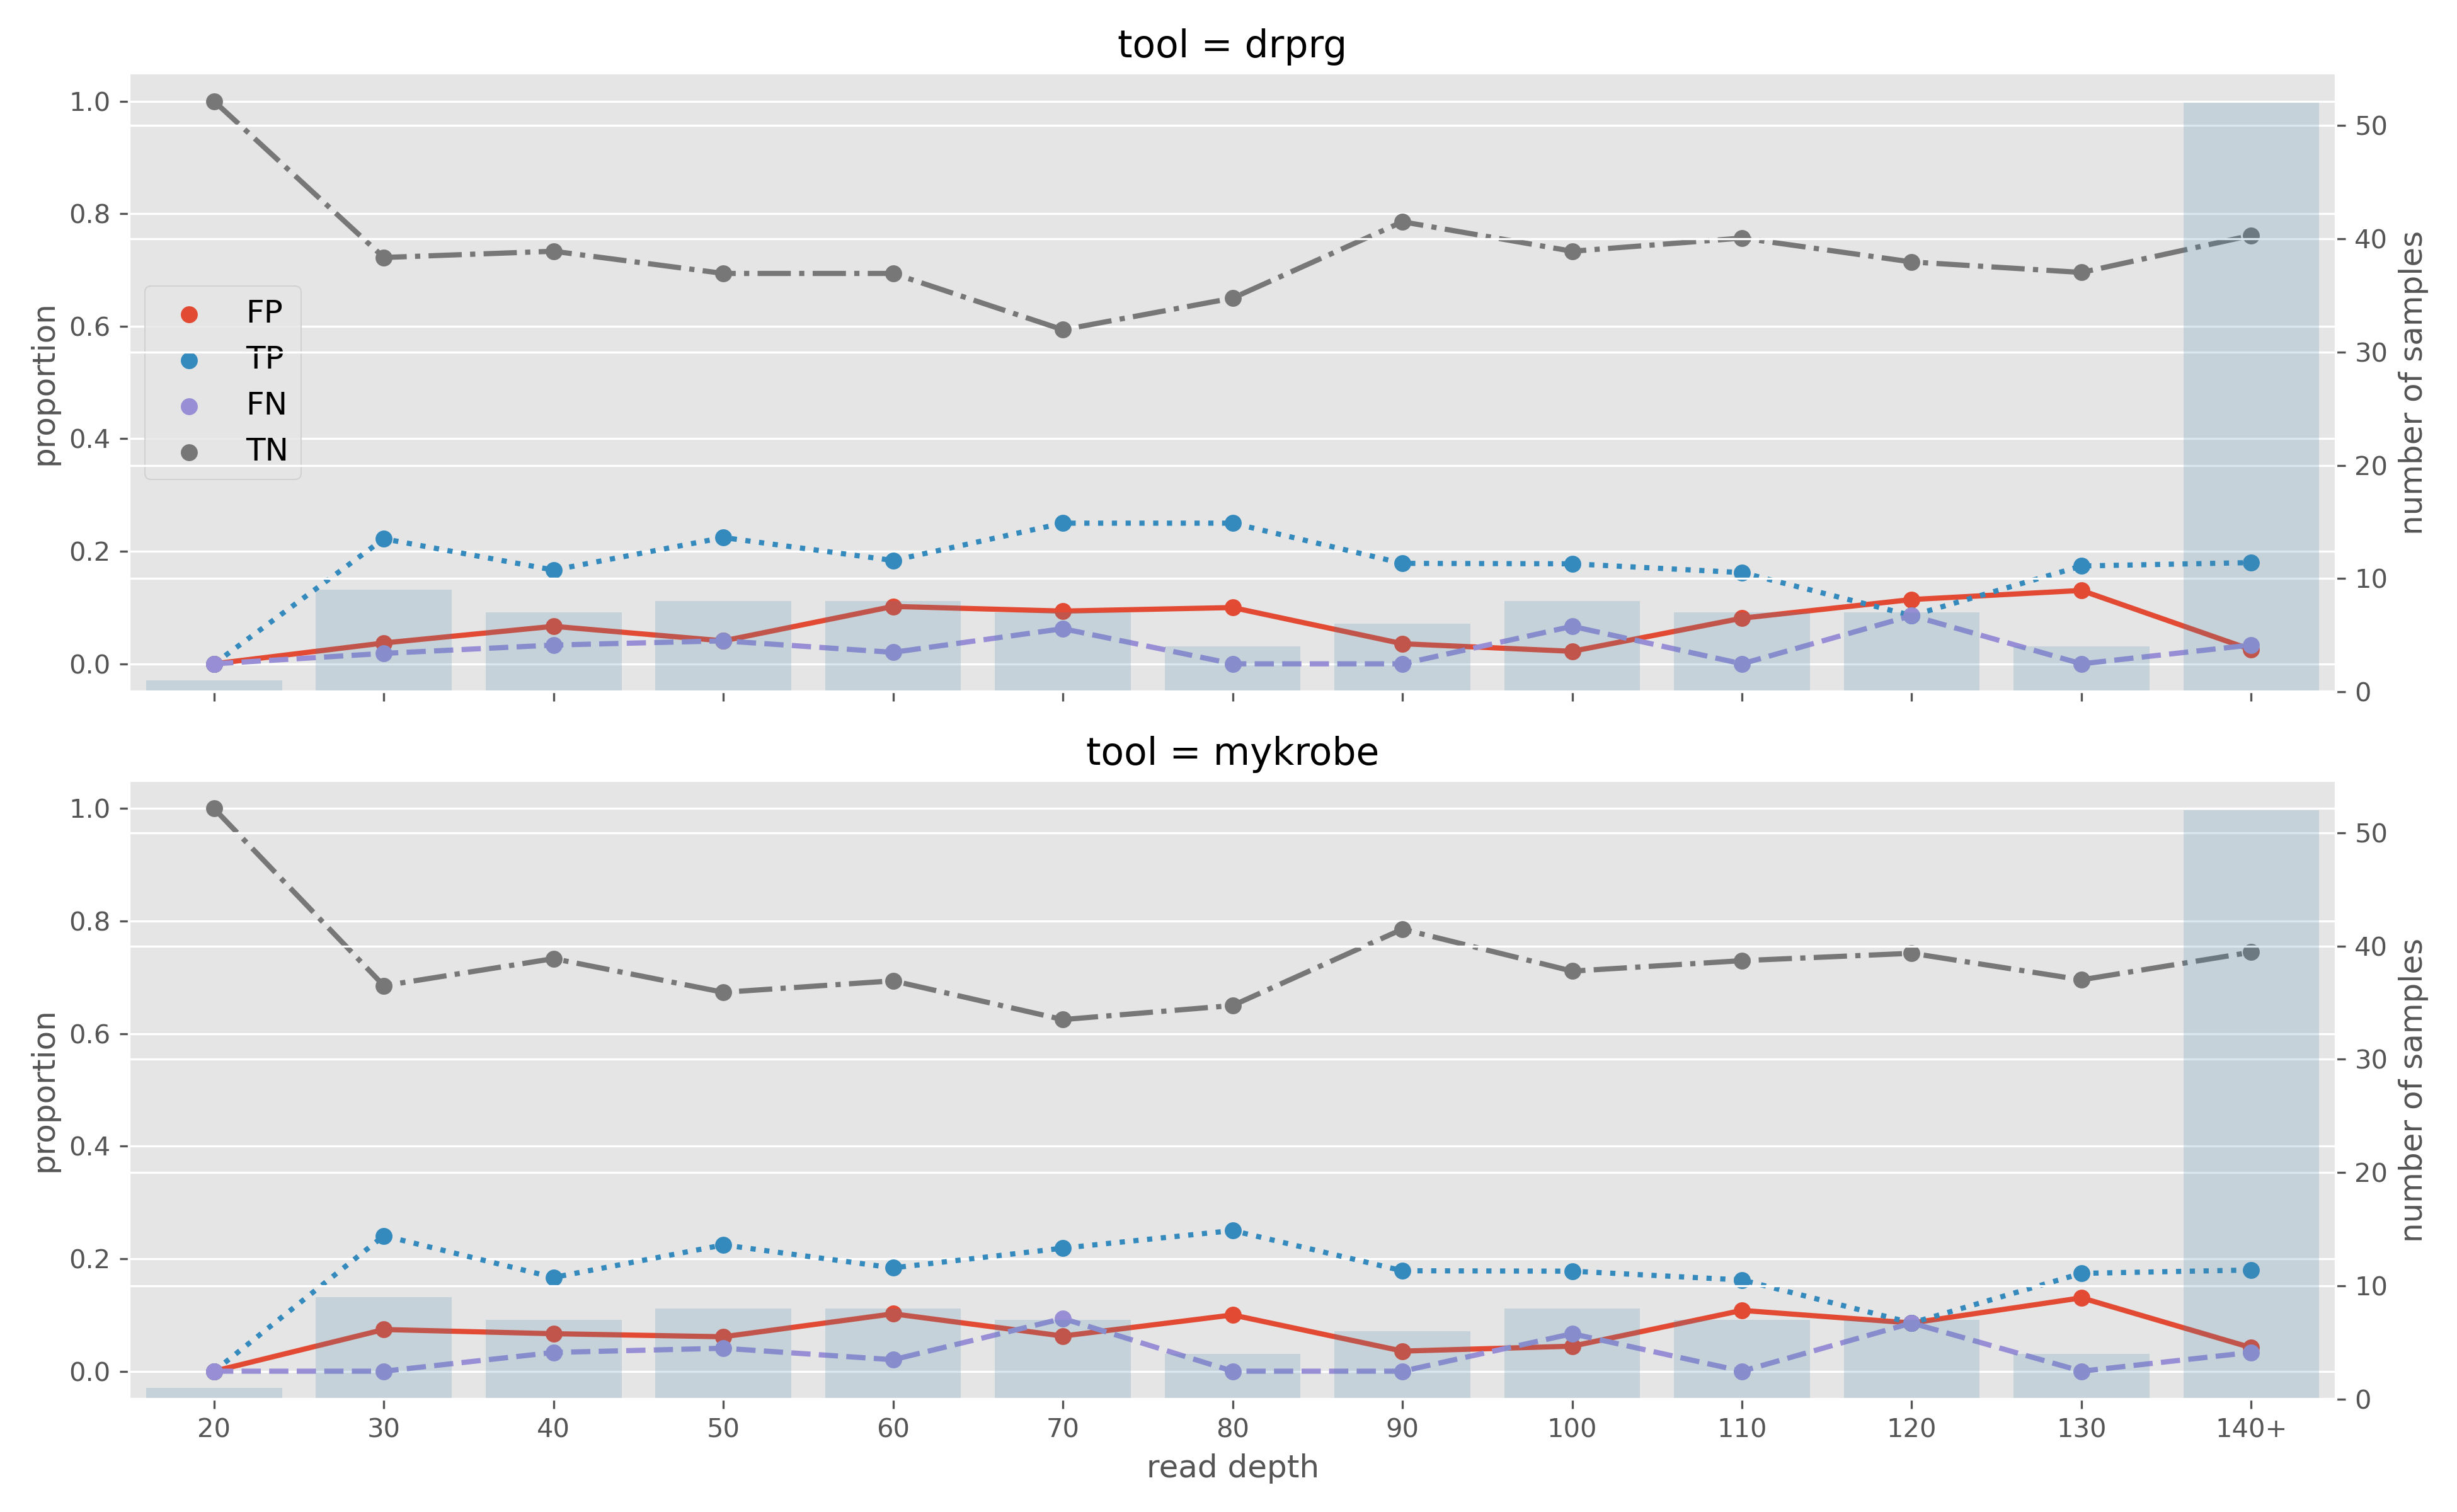
\includegraphics[width=0.90\columnwidth]{Chapter3/Figs/phenotype_coverage.png}
\caption{{Effect of Nanopore read depth on drprg (top) and mykrobe (bottom) phenotype prediction. Each point indicates the proportion (y-axis) of classifications of that type at the read depth (x-axis). Read depth is "binned". That is, read depth 40 is all samples with a read depth greater than 40 and less than or equal to 50. FP - false positive; TN - true negative; etc.
{\label{fig:pheno-covg}}
}}
\end{center}
\end{figure}
%=========================================================================
\section{Flagging novel variants not in panel}
%  what impact does this have on previous results
% http://www.crypticproject.org/wp-content/uploads/2018/09/Prediction-of-Susceptibility-to-First-Line-Tuberculosis-Drugs-by-DNA-Sequencing.pdf
% i guess what might be important here is whether FNs on phenotype are "fixed" by finding novel variants. Look through compass and bcftools VCFs for SNPs not in the panel
% we could also remove some common variants from the panel and see what difference novel would have then
% https://pubmed.ncbi.nlm.nih.gov/27436385/ shows lots of unknown mutations in gid, which we have a lot of novel variants for

%=========================================================================
\section{Discussion}

%=========================================================================
\section{Conclusion}

%=========================================================================
\section{Future work}

%=========================================================================
\section{Availability of data and materials}